
\section{Понятия окисления и восстановления. Типичные восстановители и окислители. Составление уравнений окислительно-восстановительных реакций: методы электронного и электронно-ионного баланса.}

Окислительно-восстановительная реакция состоиз из двух полуреакций --- восстановления и оксиления.\\

\textbf{Восстановитель} --- элемент, который теряет электроны (увеличивает степень окисления) --- \textit{оксиляется}.\\

\textbf{Окислитель} --- элемент, который получает электроны (уменьшает степень окисления) --- \textit{восстаноавливается}.\\

Окислителем и восстановителем также называют вещества-реагенты, содержащие соответсвтующие элементы.

\begin{figure}[H]
	\centering
	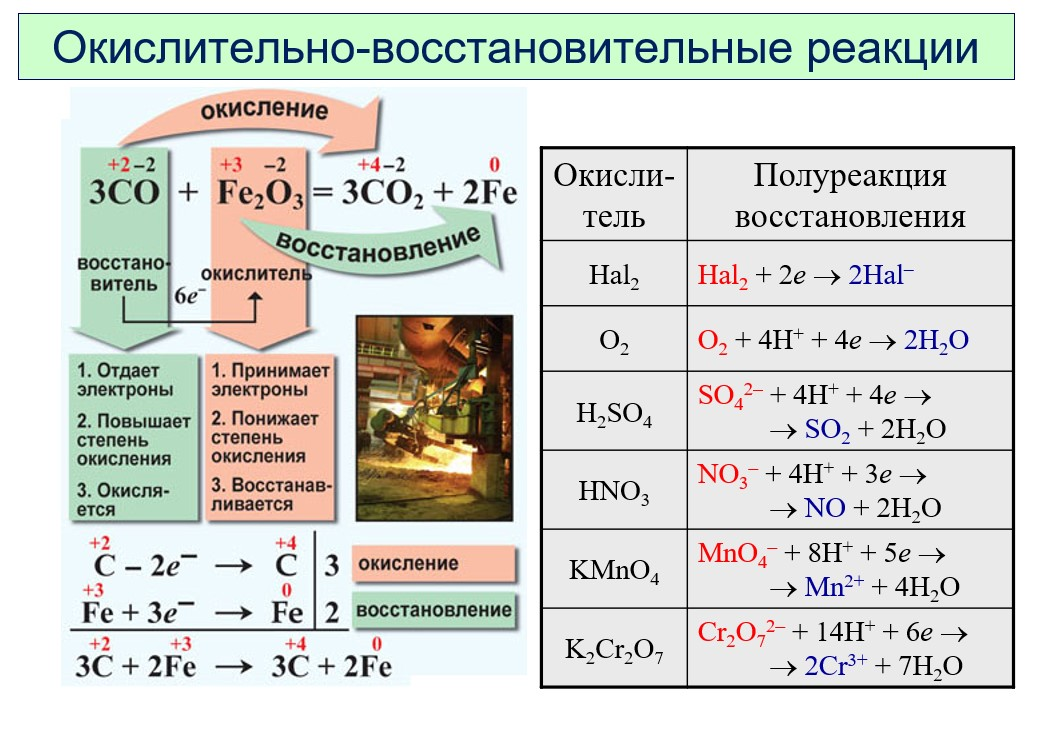
\includegraphics[width=\linewidth]{Pictures/Il1.jpg}
	\caption{Слайды Ильяса --- вместо тысячи слов.}
	\label{fig:Il1}
\end{figure}

\subsection{Типичные окислители и восстановители}

\begin{figure}[H]
	\centering
	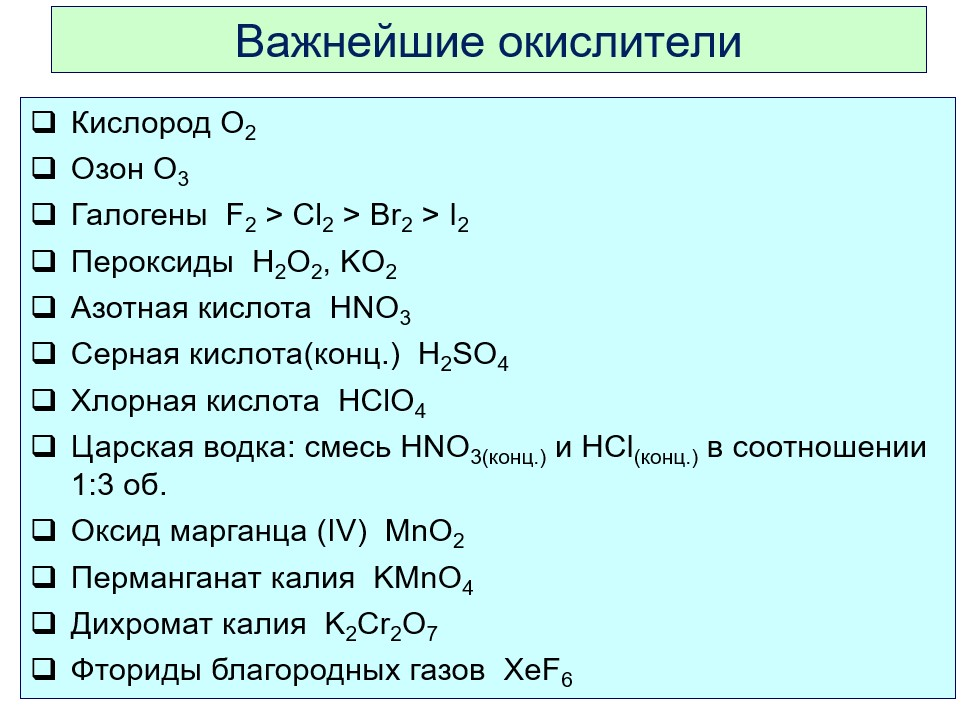
\includegraphics[width=0.7\linewidth]{Pictures/Il2.jpg}
	\caption{Окислители.}
\end{figure}
\begin{figure}[H]
	\centering
	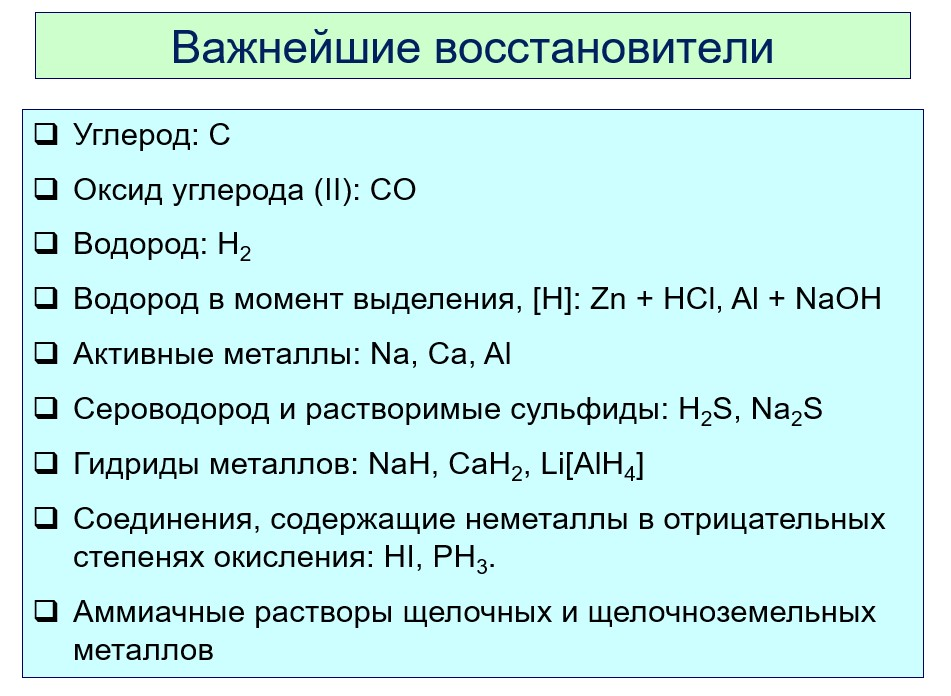
\includegraphics[width=0.7\linewidth]{Pictures/Il3.jpg}
	\caption{Восстановители.}
\end{figure}

\subsection{Методы электронного и электронно-ионного баланса}

В методе \textbf{электронного баланса} рассматривают переход электронов между элементами в определенных степенях окисления:

\begin{itemize}
	\item У кислорода всегда степень окисления -2
	\item У фтора всегда -1
	\item У водорода в соединениях с неметаллами +1, с металлами -1.
	\item У простых веществ всегда ноль.
	\item Степень окисления металлов всешда положительна. У металлов сновной группы равна её номеру, у металлов побочной может принимать разные значеия.
	\item Максимальная положиельная степеь окисления равна номеру группы
	\item Сумма степеней окисления элементов в атоме равна 0\\

\end{itemize}
	
Смотрим, какие элементы меняют степень окисления (кто отдает и кто принимает эелектроны), далее по количеству электронов уравниваем реакцию, как в примере на картинке \ref{fig:Il1}.\\

\textbf{Метод электронно-ионного баланса}

Отличается тем, что учтитывается кислотность/щёлочность/нейтральность среды.

\begin{figure}[H]
	\centering
	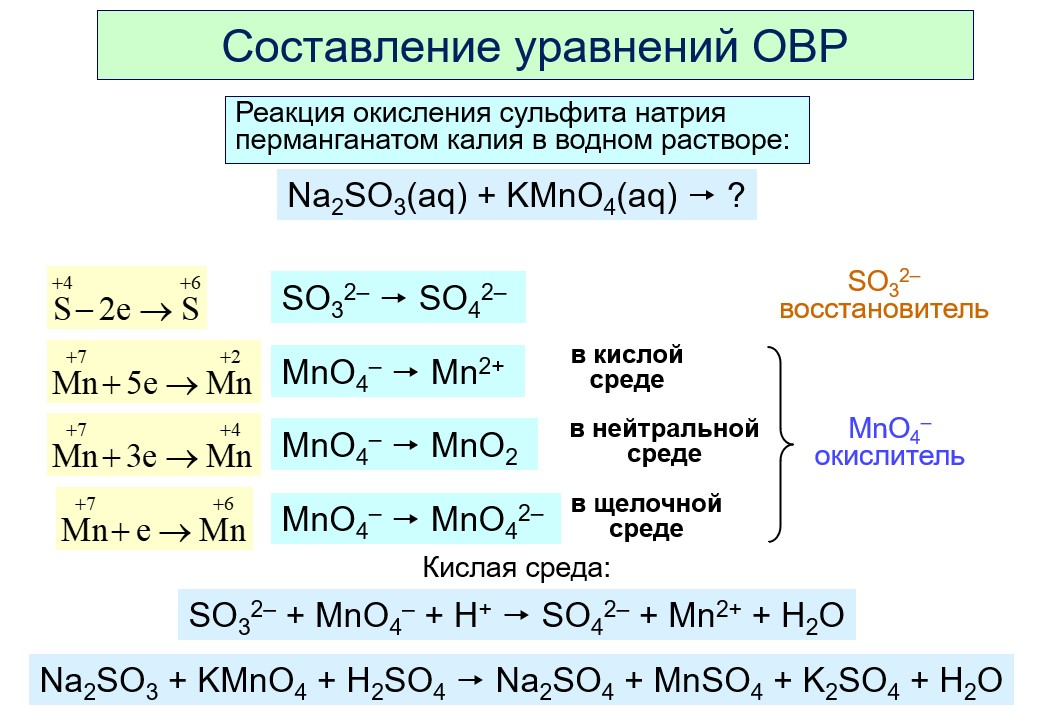
\includegraphics[width=\linewidth]{Pictures/El1.jpg}
	\caption{Составление ОВР с учетом среды.}
\end{figure}
\begin{figure}[H]
	\centering
	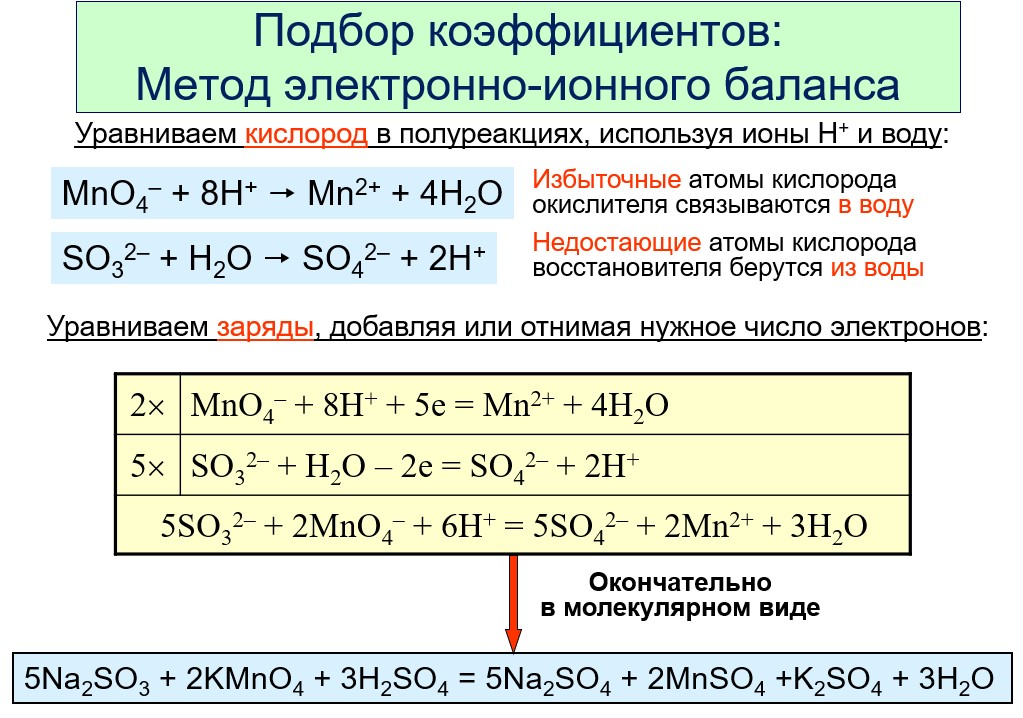
\includegraphics[width=\linewidth]{Pictures/El2.jpg}
	\caption{Подбор коэффициентов и молекулярное уравнение.}
\end{figure}
\begin{figure}[H]
	\centering
	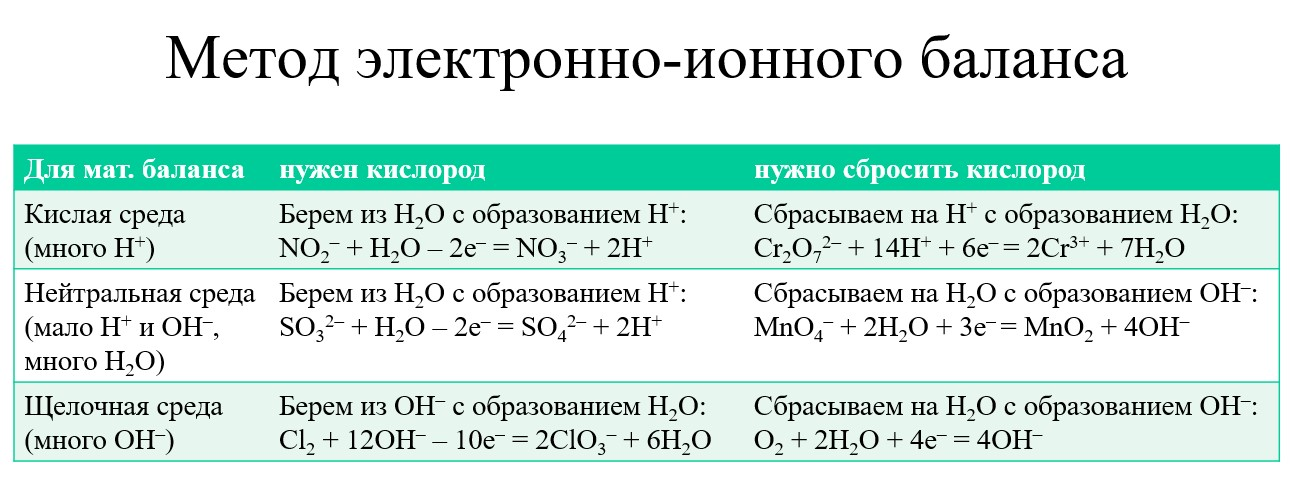
\includegraphics[width=\linewidth]{Pictures/El3.jpg}
	\caption{Памятка о нахождении и сбросе кислорода с учетом среды.}
\end{figure}

